\documentclass{article}
\usepackage[paperheight=11in,paperwidth=15in]{geometry}

\usepackage{tikz}

%% image
\usetikzlibrary{fadings,shapes.arrows,shadows}
\tikzfading[name=arrowfading]
\tikzset{arrowfill/.style={top color=black, bottom color=black}}
\tikzset{arrowstyle/.style={draw=black,arrowfill, single arrow,minimum height=#1, single arrow,
single arrow head extend=.3cm,}}

\newcommand{\tikzfancyarrow}[2][1cm]{\tikz[baseline=-2cm]\node [arrowstyle=#1] {#2};}
\begin{document}

\newcommand*{\xMax}{4}
\newcommand*{\yMax}{3}
\newcommand*{\xMin}{0}
\newcommand*{\yMin}{0}



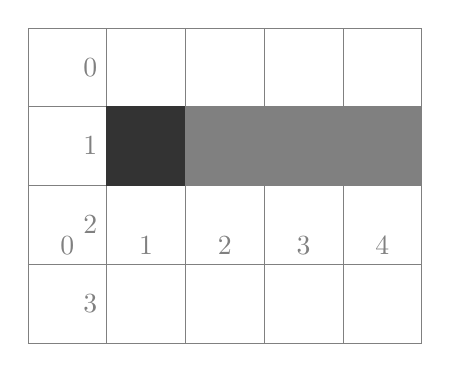
\begin{tikzpicture}

\foreach \i in {0,...,4} {
	\draw [very thin,gray] (\i,\yMin) -- (\i,\yMax)  node [above] at (\i+0.5,\yMax+1) {$\i$};
}
\foreach \i in {0,...,3} {
	\draw [very thin,gray] (\xMin,\i) -- (\xMax,\i) node [left] at (\xMin,3-\i+0.5) {$\i$};
}
\draw[step=1.0, help lines] (0, 0) grid (5,4);


\filldraw[color=black!80](1, 2) rectangle (2, 3);
\filldraw[draw=black,color=gray](2, 2) rectangle (3, 3);
\filldraw[draw=black,color=gray](3, 2) rectangle (4, 3);
\filldraw[draw=black,color=gray](4, 2) rectangle (5, 3);

\end{tikzpicture}
\tikzfancyarrow[1.5cm]{}
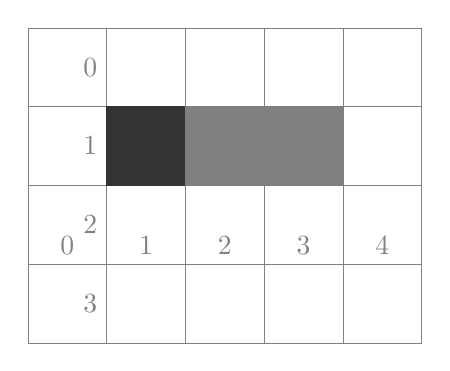
\begin{tikzpicture}

\foreach \i in {0,...,4} {
	\draw [very thin,gray] (\i,\yMin) -- (\i,\yMax)  node [above] at (\i+0.5,\yMax+1) {$\i$};
}
\foreach \i in {0,...,3} {
	\draw [very thin,gray] (\xMin,\i) -- (\xMax,\i) node [left] at (\xMin,3-\i+0.5) {$\i$};
}
\draw[step=1.0, help lines] (0, 0) grid (5,4);


\filldraw[color=black!80](1, 2) rectangle (2, 3);
\filldraw[draw=black,color=gray](2, 2) rectangle (3, 3);
\filldraw[draw=black,color=gray](3, 2) rectangle (4, 3);

\end{tikzpicture}
\tikzfancyarrow[1.5cm]{}
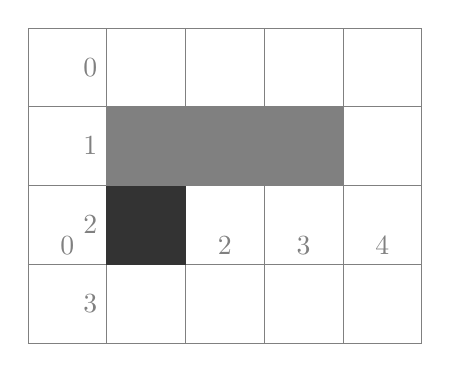
\begin{tikzpicture}

\foreach \i in {0,...,4} {
	\draw [very thin,gray] (\i,\yMin) -- (\i,\yMax)  node [above] at (\i+0.5,\yMax+1) {$\i$};
}
\foreach \i in {0,...,3} {
	\draw [very thin,gray] (\xMin,\i) -- (\xMax,\i) node [left] at (\xMin,3-\i+0.5) {$\i$};
}
\draw[step=1.0, help lines] (0, 0) grid (5,4);


\filldraw[color=black!80](1, 1) rectangle (2, 2);
\filldraw[draw=black,color=gray](1, 2) rectangle (2, 3);
\filldraw[draw=black,color=gray](2, 2) rectangle (3, 3);
\filldraw[draw=black,color=gray](3, 2) rectangle (4, 3);
\end{tikzpicture}

\hspace*{-100pt}

%% array 1
\usetikzlibrary{arrows.meta,chains,%
                    decorations.pathreplacing}
\begin{tikzpicture}[
	start chain = going right,
	node distance = 0pt,
	MyStyle/.style={draw, minimum width=2em, minimum height=2em, 
		outer sep=0pt, on chain},
	my arrow/.style={shape=single arrow, rotate=90, inner sep=1pt, outer sep=0pt, single arrow head extend=1pt, minimum height=7.5pt, text width=0pt, draw=black!50, fill=black!25}
]
\node [left=20pt, text width=20pt] (0) {row};
\node [MyStyle] (1) {$1$};
\node [MyStyle] (2) {$1$};
\node [MyStyle] (3) {$1$};
\node [MyStyle] (4) {$1$};
\begin{scope}[-{Stealth[length = 2.5pt]}]
\end{scope}
\node [above=0pt of 1.north] {[$0$]};
\node [above=0pt of 2.north] {[$1$]};
\node [above=0pt of 3.north] {[$2$]};
\node [above=0pt of 4.north] {[$3$]};

\end{tikzpicture}

\begin{tikzpicture}[
	start chain = going right,
	node distance = 0pt,
	MyStyle/.style={draw, minimum width=2em, minimum height=2em, 
		outer sep=0pt, on chain},
	my arrow/.style={shape=single arrow, rotate=90, inner sep=1pt, outer sep=0pt, single arrow head extend=1pt, minimum height=7.5pt, text width=0pt, draw=black!50, fill=black!25}
]
\node [left=20pt, text width=20pt] (0) {column};
\node [MyStyle] (1) {$1$};
\node [MyStyle] (2) {$2$};
\node [MyStyle] (3) {$3$};
\node [MyStyle] (4) {$4$};
\begin{scope}[-{Stealth[length = 2.5pt]}]
\end{scope}

\node [below=2.5pt of 1.south, anchor=east, my arrow] {};
\node [below=10.5pt of 1.south] {head};
\node [below=2.5pt of 4.south, anchor=east, my arrow] {};
\node [below=10.5pt of 4.south] {tail};

\end{tikzpicture}

%% array state 2
\begin{tikzpicture}[
	start chain = going right,
	node distance = 0pt,
	MyStyle/.style={draw, minimum width=2em, minimum height=2em, 
		outer sep=0pt, on chain},
	my arrow/.style={shape=single arrow, rotate=90, inner sep=1pt, outer sep=0pt, single arrow head extend=1pt, minimum height=7.5pt, text width=0pt, draw=black!50, fill=black!25}
]
\node [left=20pt, text width=20pt] (0) {row};
\node [MyStyle] (1) {$1$};
\node [MyStyle] (2) {$1$};
\node [MyStyle] (3) {$1$};
\node [MyStyle] (4) {$2$};
\begin{scope}[-{Stealth[length = 2.5pt]}]
\end{scope}
\node [above=0pt of 1.north] {[$0$]};
\node [above=0pt of 2.north] {[$1$]};
\node [above=0pt of 3.north] {[$2$]};
\node [above=0pt of 4.north] {[$3$]};
\end{tikzpicture}

\begin{tikzpicture}[
	start chain = going right,
	node distance = 0pt,
	MyStyle/.style={draw, minimum width=2em, minimum height=2em, 
		outer sep=0pt, on chain},
	my arrow/.style={shape=single arrow, rotate=90, inner sep=1pt, outer sep=0pt, single arrow head extend=1pt, minimum height=7.5pt, text width=0pt, draw=black!50, fill=black!25}
]
\node [left=20pt, text width=20pt] (0) {column};
\node [MyStyle] (1) {$1$};
\node [MyStyle] (2) {$2$};
\node [MyStyle] (3) {$3$};
\node [MyStyle] (4) {$1$};
\begin{scope}[-{Stealth[length = 2.5pt]}]
\end{scope}

\node [below=2.5pt of 4.south, anchor=east, my arrow] {};
\node [below=10.5pt of 4.south] {head};
\node [below=2.5pt of 3.south, anchor=east, my arrow] {};
\node [below=10.5pt of 3.south] {tail};

\end{tikzpicture}

%% Grid G
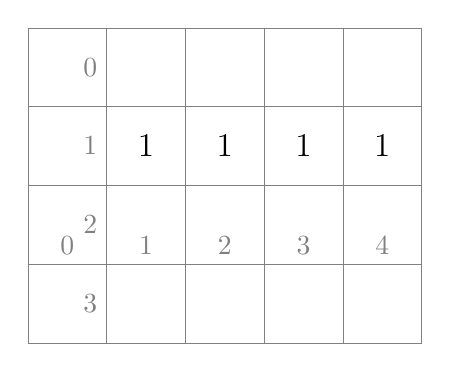
\begin{tikzpicture}

\foreach \i in {0,...,4} {
	\draw [very thin,gray] (\i,\yMin) -- (\i,\yMax)  node [above] at (\i+0.5,\yMax+1) {$\i$};
}
\foreach \i in {0,...,3} {
	\draw [very thin,gray] (\xMin,\i) -- (\xMax,\i) node [left] at (\xMin,3-\i+0.5) {$\i$};
}
\draw[step=1.0, help lines] (0, 0) grid (5,4);

\node at (1+0.5,2+0.5) {\large{1}};
\node at (2+0.5,2+0.5) {\large{1}};
\node at (3+0.5,2+0.5) {\large{1}};
\node at (4+0.5,2+0.5) {\large{1}};

\end{tikzpicture}
\tikzfancyarrow[1.5cm]{}
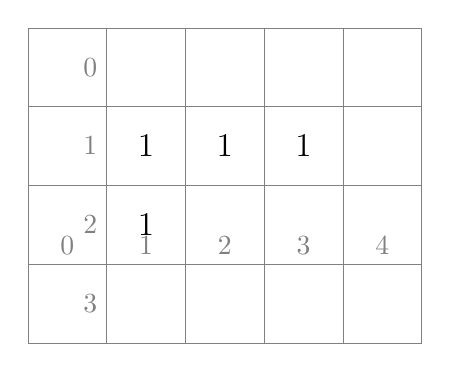
\begin{tikzpicture}

\foreach \i in {0,...,4} {
	\draw [very thin,gray] (\i,\yMin) -- (\i,\yMax)  node [above] at (\i+0.5,\yMax+1) {$\i$};
}
\foreach \i in {0,...,3} {
	\draw [very thin,gray] (\xMin,\i) -- (\xMax,\i) node [left] at (\xMin,3-\i+0.5) {$\i$};
}
\draw[step=1.0, help lines] (0, 0) grid (5,4);

\node at (1+0.5,2+0.5) {\large{1}};
\node at (2+0.5,2+0.5) {\large{1}};
\node at (3+0.5,2+0.5) {\large{1}};
\node at (1+0.5,1+0.5) {\large{1}};

\end{tikzpicture}

\end{document}
